\documentclass[a4paper,11pt]{article}

% 日本語対応
\usepackage{xeCJK}
\setCJKmainfont{Yu Gothic}

% 数学関連パッケージ
\usepackage{amsmath}
\usepackage{amssymb}
\usepackage{amsthm}
\usepackage{amsfonts}
\usepackage{mathtools}

% 図形描画用パッケージ
\usepackage{tikz}
\usepackage{pgfplots}
\pgfplotsset{compat=1.18}
\usetikzlibrary{intersections,patterns,angles,quotes,calc,fillbetween}

% その他パッケージ
\usepackage{graphicx}
\usepackage{enumitem}
\usepackage{float}
\usepackage{hyperref}
\usepackage{fancyhdr}
\usepackage{geometry}
\usepackage{xcolor}

% ページ設定
\geometry{
  a4paper,
  top=25mm,
  bottom=25mm,
  left=25mm,
  right=25mm
}

% 数式環境設定
\numberwithin{equation}{section}
\newtheorem{theorem}{定理}
\newtheorem{lemma}[theorem]{補題}
\newtheorem{proposition}[theorem]{命題}
\newtheorem{corollary}[theorem]{系}
\theoremstyle{definition}
\newtheorem{definition}[theorem]{定義}
\newtheorem{example}[theorem]{例}
\newtheorem{exercise}{問題}
\theoremstyle{remark}
\newtheorem*{remark}{注意}
\newtheorem*{solution}{解答}

% ヘッダーとフッターの設定
\pagestyle{fancy}
\fancyhf{}
\fancyhead[L]{数学問題}
\fancyhead[R]{\today}
\fancyfoot[C]{\thepage}
\renewcommand{\headrulewidth}{0.4pt}
\renewcommand{\footrulewidth}{0.4pt}

% タイトル情報
\title{数学問題}
\author{数学問題生成AIシステム}
\date{\today}

% ドキュメント開始
\begin{document}

\maketitle

% 問題セクション
\section*{問題}

% 問題文を挿入(変数で置換)
2次関数 $f(x) = 3x^2 - 6x + 2$ の頂点の座標を求めよ。

% 図形が必要な場合はここに挿入
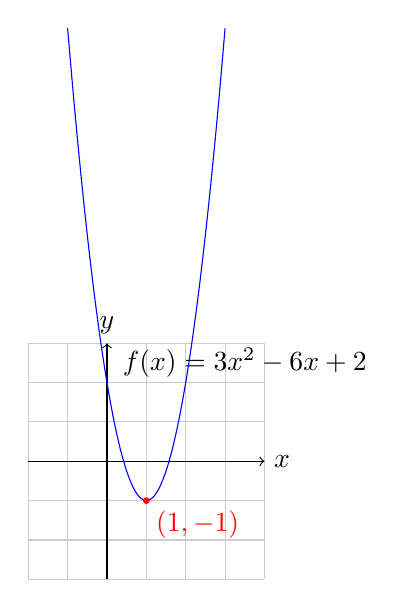
\begin{tikzpicture}[scale=0.5]
  % Draw axes
  \draw[thin,gray!40] (-2,-3) grid (4,3);
  \draw[->] (-2,0)--(4,0) node[right]{$x$};
  \draw[->] (0,-3)--(0,3) node[above]{$y$};

  % Draw function
  \draw[domain=-1:3,smooth,variable=\x,blue] plot ({\x},{3*\x*\x - 6*\x + 2});

  % Draw vertex
  \filldraw [red] (1,-1) circle (2pt) node[anchor=north west] {$(1, -1)$};

  % Label the function
  \node at (3.5,2.5) {$f(x) = 3x^2 - 6x + 2$};
\end{tikzpicture}

% 解答セクション(オプショナル - 表示したくない場合はコメントアウト)
\section*{解答}

% 解答を挿入(変数で置換)
$(1, -1)$

% 解説セクション(オプショナル - 表示したくない場合はコメントアウト)
\section*{解説}

% 解説を挿入(変数で置換)
二次関数の頂点の座標は公式 $\left(-\frac{b}{2a}, f\left(-\frac{b}{2a}\right)\right)$ で求めることができる。ここで、$a = 3$、$b = -6$、$c = 2$ であるから、$-\frac{b}{2a} = \frac{-(-6)}{2 \cdot 3} = 1$ となる。次に、$f(1) = 3(1)^2 - 6 \cdot 1 + 2 = 3 - 6 + 2 = -1$ を計算する。よって、頂点の座標は $(1, -1)$ である。

\end{document} 